\documentclass[11pt,a4paper]{article}
\usepackage[utf8]{inputenc}
\usepackage[T1]{fontenc}
\usepackage[spanish]{babel}
\usepackage[margin=2cm]{geometry}
\usepackage{booktabs}
\usepackage{array}
\usepackage{multirow}
\usepackage{xcolor}
\usepackage{colortbl}
\usepackage{graphicx}
\usepackage{hyperref}
\usepackage{parskip}
\usepackage{tcolorbox}
\usepackage{enumitem}

\definecolor{accent}{HTML}{1f77b4}
\definecolor{good}{HTML}{2ca02c}
\definecolor{bad}{HTML}{d62728}
\definecolor{lightgray}{HTML}{F2F2F2}
\definecolor{boxbg}{HTML}{EAF3FB}

\hypersetup{colorlinks=true, urlcolor=accent}

\title{\vspace{-2.5em}\textbf{An\'alisis exploratorio del fraud\_dataset}\\
       \large{Conclusiones para la presentaci\'on -- Ejercicio 1}}
\author{SIA TP3 -- ITBA 1Q 2026}
\date{}

\newtcolorbox{takeaway}{colback=boxbg, colframe=accent, boxrule=0.5pt,
  arc=2pt, left=8pt, right=8pt, top=4pt, bottom=4pt}

\begin{document}
\maketitle
\vspace{-1.5em}

\section{Contexto y dataset}

El \texttt{fraud\_dataset.csv} contiene \textbf{7500 transacciones} con 9 features y dos
columnas relacionadas al target:
\begin{itemize}[leftmargin=*, itemsep=2pt, topsep=2pt]
    \item \texttt{big\_model\_fraud\_probability} ($\in [0,1]$): salida del BigModel,
          es lo que el TinyModel debe \emph{replicar} (knowledge distillation).
    \item \texttt{flagged\_fraud} ($\in \{0,1\}$): ground truth, \textbf{solo para evaluaci\'on}
          (no se usa para entrenar).
\end{itemize}

\textbf{Distribuci\'on de clases:} 869 fraudes (11.59\%) vs 6631 leg\'itimas (88.41\%).
Existe \textbf{desbalance} relevante para la elecci\'on del umbral final y para
las m\'etricas que conviene reportar.

\section{Vista general: scatter feature vs target}

Para cada feature graficamos su relaci\'on con \texttt{big\_model\_fraud\_probability},
coloreando por \texttt{flagged\_fraud} (azul = leg\'itimo, rojo = fraude real).

\begin{center}
  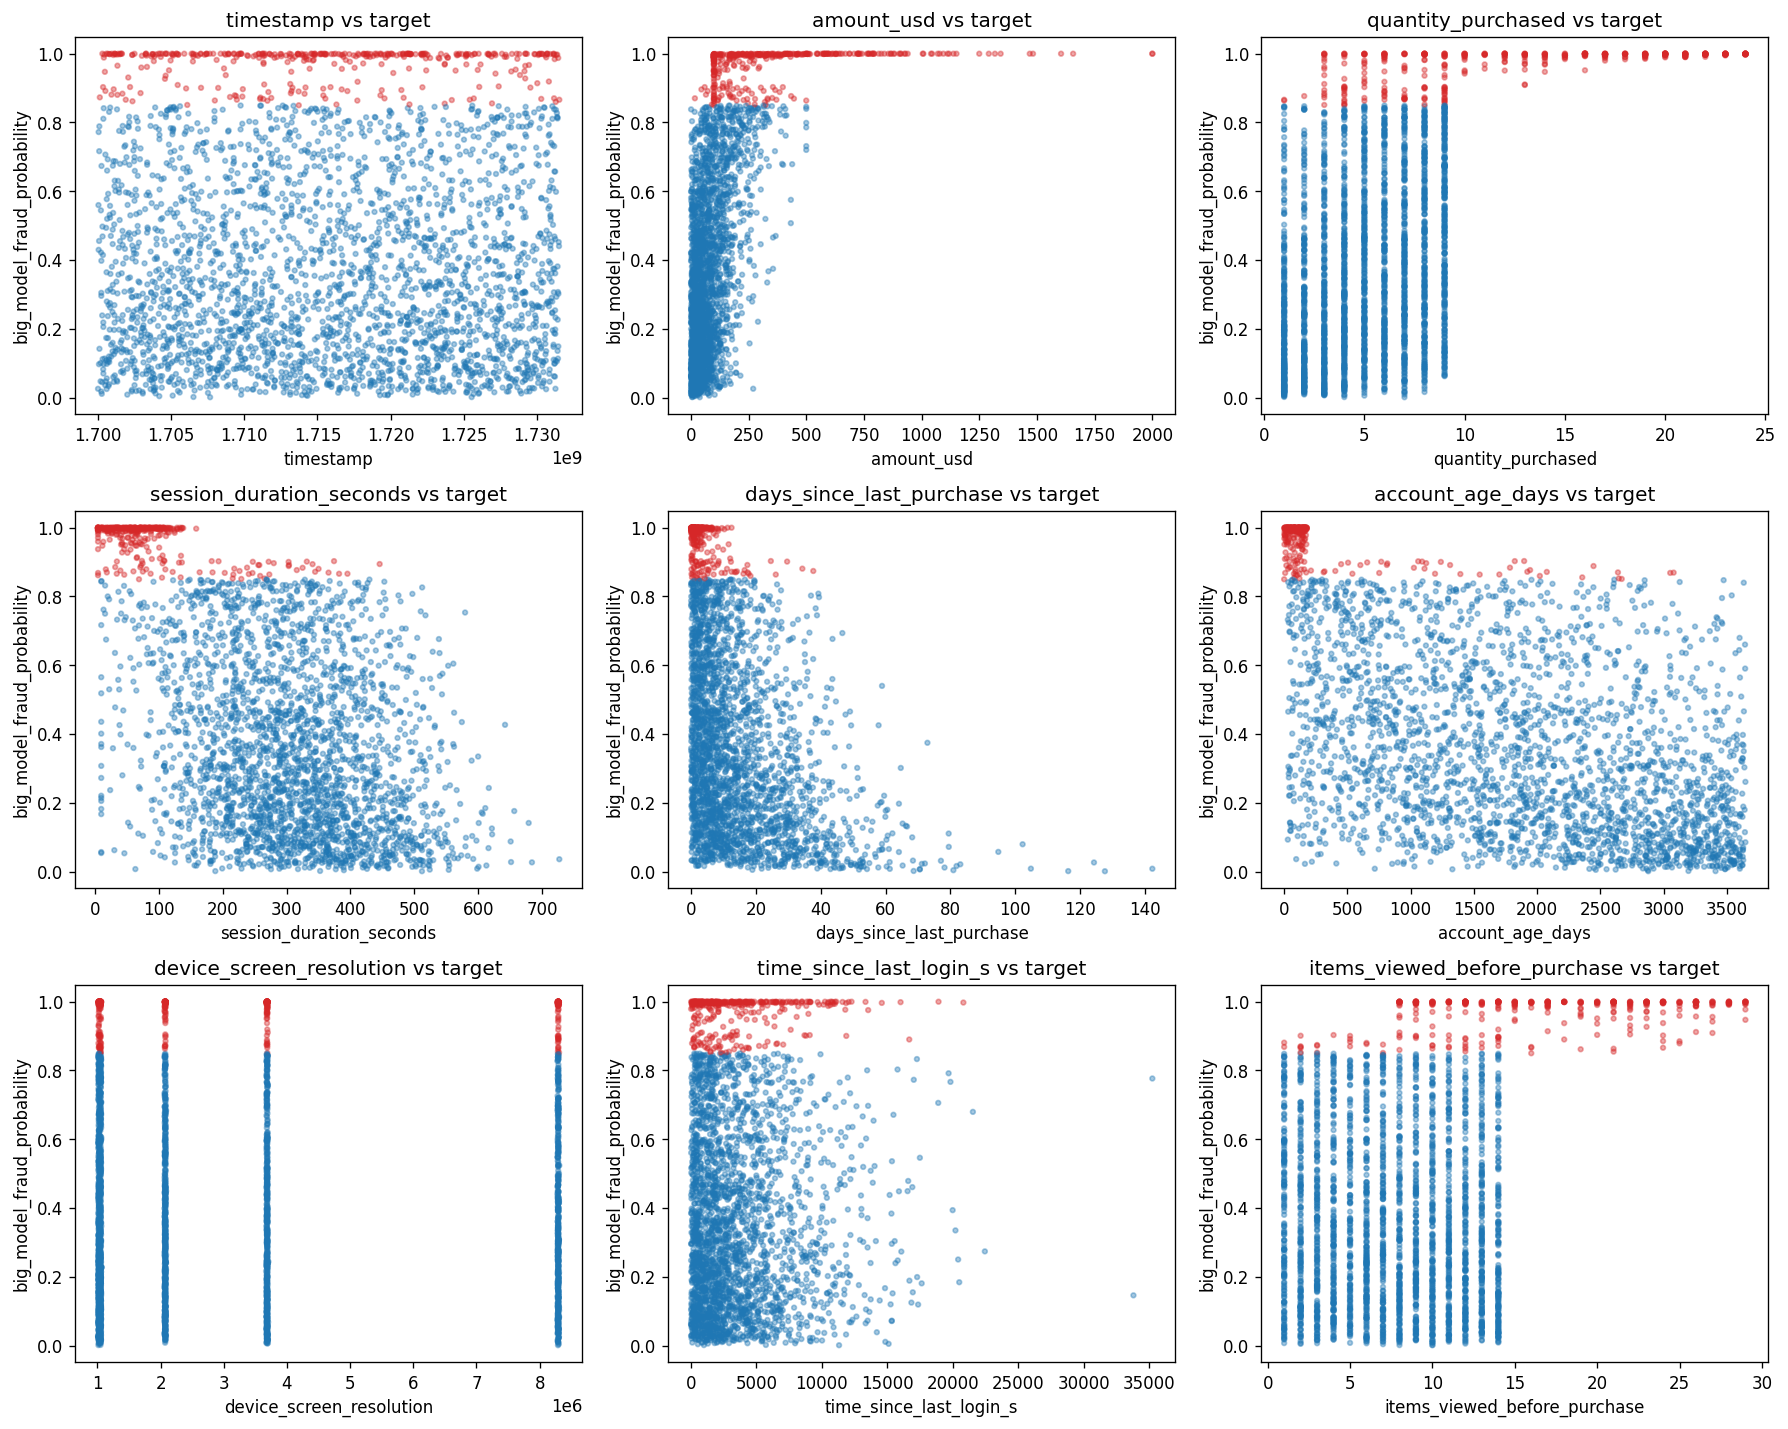
\includegraphics[width=\textwidth]{scatter_grid.png}
\end{center}

\begin{takeaway}
\textbf{Observaciones a primera vista:}
\begin{itemize}[leftmargin=*, itemsep=1pt, topsep=2pt]
    \item En \texttt{amount\_usd}, \texttt{quantity\_purchased} e
          \texttt{items\_viewed\_before\_purchase}, los puntos rojos
          (fraude) ocupan exclusivamente la parte derecha del eje X. Hay
          \textbf{umbrales duros} a partir de los cuales \emph{todo} es fraude.
    \item \texttt{account\_age\_days} muestra dos modos casi disjuntos: el rojo
          se concentra a la izquierda, el azul a la derecha.
    \item \texttt{timestamp}, \texttt{device\_screen\_resolution} y
          \texttt{time\_since\_last\_login\_s} muestran nubes mezcladas
          sin estructura aparente: ambos colores se solapan en todo el rango.
\end{itemize}
\end{takeaway}

\section{Hallazgo principal: tres reglas determin\'isticas}

Tres features tienen \textbf{umbrales que separan perfectamente} las clases en el
dataset. Combinadas como OR:

\begin{center}
\fbox{\parbox{0.85\textwidth}{\centering
\texttt{amount\_usd > 500} $\;\lor\;$ \texttt{quantity\_purchased $\geq$ 10} $\;\lor\;$ \texttt{items\_viewed\_before\_purchase $\geq$ 15}}}
\end{center}

\subsection{Aporte de cada regla individual}

\begin{center}
\begin{tabular}{l c c c}
\toprule
\textbf{Regla} & \textbf{Matches} & \textbf{TP} & \textbf{FP} \\
\midrule
\texttt{amount\_usd > 500}                          & 199 & 199 & 0 \\
\texttt{quantity\_purchased $\geq$ 10}              & 524 & 524 & 0 \\
\texttt{items\_viewed\_before\_purchase $\geq$ 15}  & 490 & 490 & 0 \\
\bottomrule
\end{tabular}
\end{center}

Las matches se solapan: las tres reglas juntas marcan \textbf{695 filas \'unicas}.

\subsection{Resultados de aplicar las reglas como predictor (\texttt{simple\_prediction})}

\begin{center}
\renewcommand{\arraystretch}{1.4}
\begin{tabular}{c c | >{\columncolor{lightgray}}c >{\columncolor{lightgray}}c}
 & & \multicolumn{2}{c}{\textbf{Predicci\'on}} \\
 & & 1 (fraude) & 0 (no fraude) \\
\hline
\multirow{2}{*}{\textbf{Real}} & 1 (fraude)    & \textcolor{good}{\textbf{TP = 695}}  & \textcolor{bad}{\textbf{FN = 174}}  \\
                                & 0 (no fraude) & \textcolor{bad}{\textbf{FP = 0}}     & \textcolor{good}{\textbf{TN = 6631}} \\
\end{tabular}
\quad
\renewcommand{\arraystretch}{1.3}
\begin{tabular}{l r}
\toprule
\textbf{M\'etrica} & \textbf{Valor} \\
\midrule
Accuracy            & \textbf{97.68\%} \\
Precision           & \textbf{100.00\%} \\
Recall              & \textbf{79.98\%} \\
\bottomrule
\end{tabular}
\end{center}

\textbf{Regla descartada:} \texttt{session\_duration\_seconds > 500} captura 1 TP
y 350 FP. Romper\'ia la precision perfecta a cambio de un solo fraude m\'as,
por lo que se descarta.

\begin{takeaway}
\textbf{El 80\% del fraude se etiqueta correctamente con tres \texttt{if}}, sin
un solo falso positivo. El \textbf{20\% restante (174 casos)} es el verdadero
desaf\'io del perceptr\'on: son fraudes que respetan los tres umbrales y solo
se detectan combinando features continuas.
\end{takeaway}

\section{Conclusiones por feature}

\begin{center}
\renewcommand{\arraystretch}{1.25}
\begin{tabular}{l r l}
\toprule
\textbf{Feature} & \textbf{Pearson r} & \textbf{Hallazgo principal} \\
\midrule
\texttt{account\_age\_days}              & $-0.585$ & Cuentas $<250$ d\'ias contienen 87.8\% del fraude \\
\texttt{quantity\_purchased}             & $+0.563$ & $\geq 10$ unidades: \textbf{100\% fraude} (524 filas) \\
\texttt{amount\_usd}                     & $+0.557$ & $> \$500$: \textbf{100\% fraude} (199 filas) \\
\texttt{session\_duration\_seconds}      & $-0.514$ & 89.1\% del fraude tiene sesi\'on $<150$s \\
\texttt{days\_since\_last\_purchase}     & $-0.404$ & 84.5\% del fraude con $<5$ d\'ias entre compras \\
\texttt{items\_viewed\_before\_purchase} & $+0.334$ & $\geq 15$ items: \textbf{100\% fraude} (490 filas) \\
\midrule
\rowcolor{lightgray}\texttt{timestamp}                & $+0.001$ & Sin se\~nal lineal ni mon\'otona \\
\rowcolor{lightgray}\texttt{device\_screen\_resolution} & $+0.025$ & Sin se\~nal lineal ni mon\'otona \\
\rowcolor{lightgray}\texttt{time\_since\_last\_login\_s} & $+0.002$ & Sin se\~nal lineal ni mon\'otona \\
\bottomrule
\end{tabular}
\end{center}

\textbf{Detalles relevantes:}
\begin{itemize}[leftmargin=*, itemsep=2pt, topsep=2pt]
    \item Las cuentas \emph{nuevas} ($<250$ d\'ias) son 87.8\% del fraude pero solo 5.7\% de las leg\'itimas.
          Las cuentas \emph{viejas} ($>1500$ d\'ias) son 59.8\% de las leg\'itimas y 0.9\% del fraude.
    \item En \texttt{days\_since\_last\_purchase}, el patr\'on ``compra reciente $\to$ probable fraude''
          es t\'ipico de uso de tarjeta robada (testeo + cargo grande en poco tiempo).
    \item Cuando hay fraude con sesi\'on corta ($<150$s), el BigModel est\'a \textbf{muy confiado}
          (mediana de probabilidad $= 0.997$): se\~nal fuerte que el TinyModel deber\'ia replicar.
    \item Las tres reglas duras son \textbf{discontinuidades}: en \texttt{quantity}, la tasa de fraude
          salta de $\sim 8\%$ en $q=9$ a $100\%$ en $q=10$. Lo mismo en $items: 14 \to 15$.
\end{itemize}

\section{Decisi\'on: features a excluir del entrenamiento}

\textbf{Tres features se descartan} del set de entrenamiento del perceptr\'on
simple del Ej 1: \texttt{timestamp}, \texttt{device\_screen\_resolution} y
\texttt{time\_since\_last\_login\_s}.

\paragraph{Validaci\'on con tres tests independientes:}

\begin{center}
\begin{tabular}{l r r r}
\toprule
\textbf{Feature} & \textbf{Pearson} & \textbf{Spearman} & \textbf{Spread media-target / decil} \\
\midrule
\texttt{timestamp}                  & $+0.001$ & $+0.004$ & 0.053 \\
\texttt{device\_screen\_resolution} & $+0.025$ & $+0.029$ & 0.051 \\
\texttt{time\_since\_last\_login\_s} & $+0.002$ & $+0.001$ & 0.021 \\
\bottomrule
\end{tabular}
\end{center}

\begin{itemize}[leftmargin=*, itemsep=2pt, topsep=2pt]
    \item \textbf{Pearson $\approx 0$:} no hay relaci\'on \emph{lineal}.
    \item \textbf{Spearman $\approx 0$:} tampoco hay relaci\'on \emph{mon\'otona}.
    \item \textbf{Media del target por decil $\approx$ constante} (alrededor del 0.42 global).
          Spread m\'aximo de 5\%, dentro del ruido estad\'istico para $\sim 750$ muestras por decil.
\end{itemize}

Adem\'as, dos de las tres features tienen magnitudes problem\'aticas (\texttt{timestamp}
en 1.7e9, \texttt{device\_screen\_resolution} en 1e6) que dominar\'ian el c\'alculo
del gradiente si no se normalizaran perfectamente.

\paragraph{Salvedad:} Esta exclusi\'on aplica al \textbf{perceptr\'on simple} del Ej 1.
Para un MLP (Ej 2/3), dos features con $r \approx 0$ podr\'ian aportar en
\emph{interacci\'on} (\textit{e.g.} $y = x_1 \cdot x_2$). Conviene reevaluar esta
decisi\'on al pasar a redes con capas ocultas.

\section{Implicancias para el TinyModel}

\begin{takeaway}
\begin{enumerate}[leftmargin=*, itemsep=3pt, topsep=2pt]
    \item \textbf{L\'inea de base obligatoria:} cualquier perceptr\'on debe
          \textbf{al menos igualar} a \texttt{simple\_prediction} (recall $\geq 80\%$,
          precision $\geq 100\%$ sobre los casos cubiertos por las reglas).
          Si no la iguala, hay un problema de capacidad o de normalizaci\'on.
    \item \textbf{Valor agregado del modelo:} se mide en cu\'antos de los \textbf{174 fraudes
          ``sutiles''} logra recuperar.
    \item \textbf{Lineal vs no-lineal:} las tres discontinuidades duras (saltos de
          $\sim 6\%$ a $100\%$ en un solo entero) son geom\'etricamente imposibles
          de reproducir con una recta. Es donde el \textbf{perceptr\'on no-lineal con
          sigmoide} debe mostrar su ventaja respecto al lineal puro.
    \item \textbf{M\'etricas:} con 88\% de no-fraude, accuracy se infla sola.
          Reportar siempre \emph{precision}, \emph{recall} y curva ROC.
    \item \textbf{Set de features final:} \texttt{account\_age\_days},
          \texttt{quantity\_purchased}, \texttt{amount\_usd},
          \texttt{session\_duration\_seconds}, \texttt{days\_since\_last\_purchase},
          \texttt{items\_viewed\_before\_purchase} (6 features informativas).
\end{enumerate}
\end{takeaway}

\end{document}
